\section{Reward Learning Algorithm}\label{sec:reward}
% \section{Segments to Rewards}
The next problem is to use the learned goals $G$ to construct rewards for the task.

\subsection{Augmentation}
The partitioning of a task requires understanding how the sub-tasks are sequentially coupled.
Therefore, during learning, the agent needs to be aware of its overall global progress.
We will show that we have to also include a vector of additional states $v$ as a state-space $\binom{s}{v}$ to account for these constraints.

The key idea is to use $G$ to concisely encode the history of process until a time $t$ in terms of previously completed sub-tasks. 
The result will be stored in a vector $v$, which the agent can use in forward RL.
Algorithm \ref{alg:tsh3} summarizes this process.
$v = e(H_t)$ is the vector that we use to augment the state-space of the RL problem.

\begin{algorithm}[t]
\small
\DontPrintSemicolon
\caption{Transition State Encoding \label{alg:tsh3}}
\KwData{Set of transition state clusters:$G$}
\KwData{Sequence of previously visited states: $H_t$}

$e \leftarrow [0,...,0]$

\ForEach{$(x,t) \in H_t$}{
   \If{$(x,t) \in$  \texttt{conf}(G)}{
      $i \leftarrow$ \texttt{find}(G,(x,t))
      
      $e[i] \leftarrow 1 \text{ if } e(i-1) = 1 \text{ or } i=0$
   }
}



\KwResult{Vector indicating which transition states where previously visited $v$}
\end{algorithm}


\subsection{Maximum Entropy Inverse Reinforcement Learning}
We use a technique called Maximum Entropy Inverse Reinforcement Learning (MaxEnt-IRL). 
MaxEnt-IRL uses the principle of maximum entropy, i.e., given some testable property select the maximum entropy distribution that encodes that property, to formalize the IRL problem.
For the IRL problem, this results in the following model.

\begin{figure*}[t]
\centering
 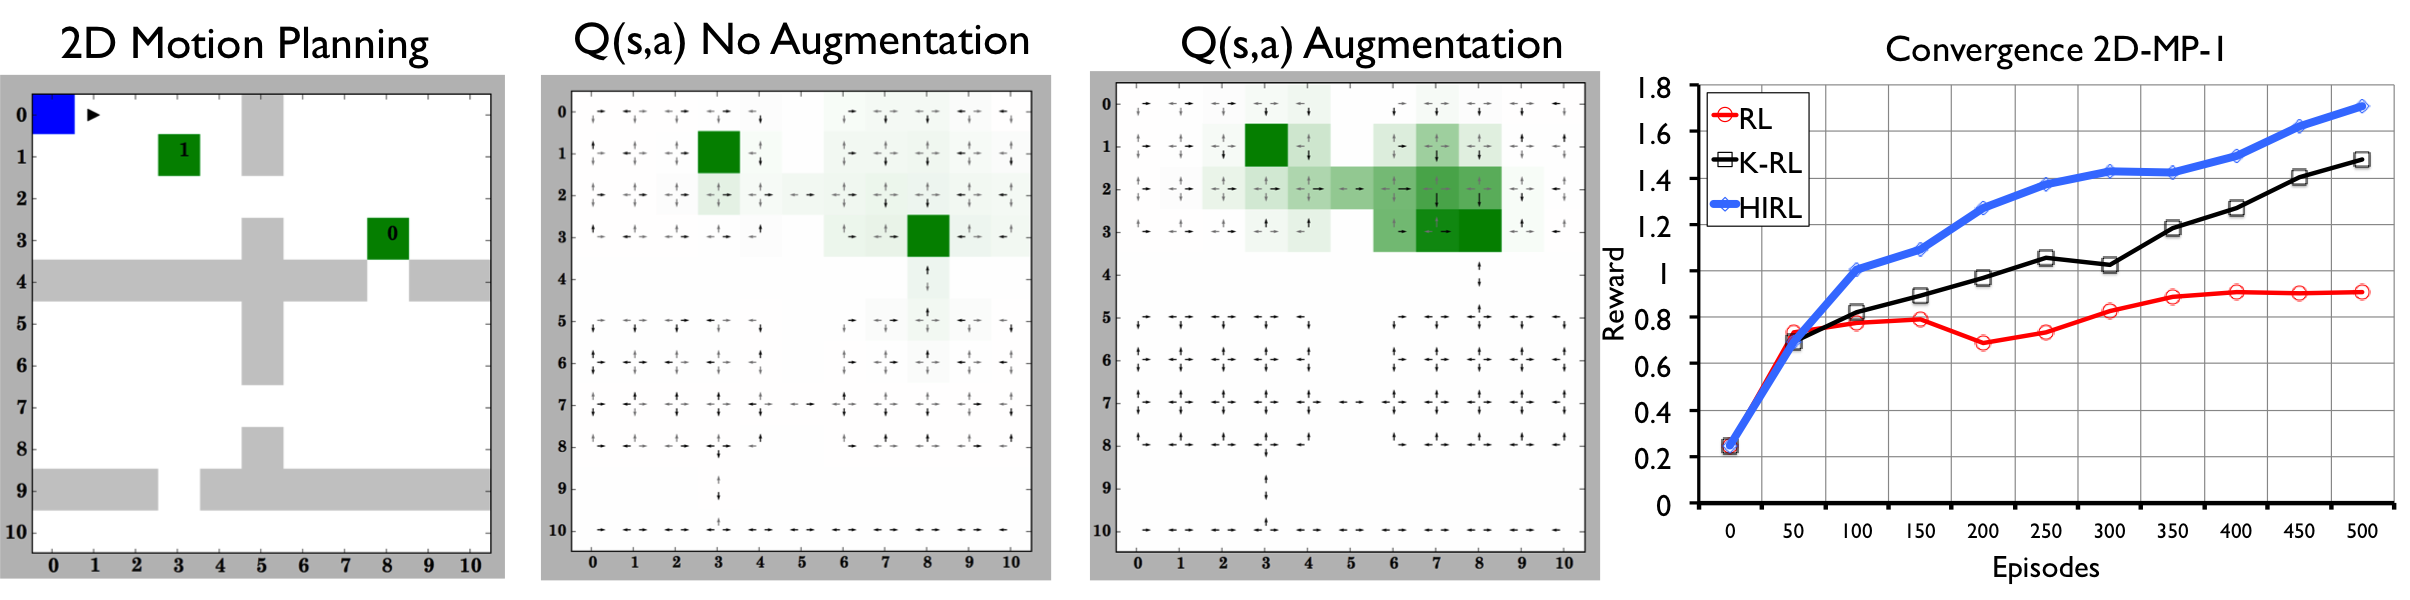
\includegraphics[width=0.8\textwidth]{exp/gw-easy-1abc.png}
 \caption{We constructed a scenario where an agent has to collect reward 0 and 1 in sequence. Since the agent has to cross over the same state in multiple stages of the task, RL can fail to converge in sequential tasks unless the state-space represents previous progress. 
 One approach is to segmented the problem into independent subtasks, which neglects any shared structure between the tasks (states far away from both goals are not valuable).
 \hirl augments the state-space with the appropriate variables and uses IRL to learn rewards that capture this structure. We plot the domain, the Q functions of the RL agent at convergence, and the learning curve (Section \ref{exp:2dmp}).  \label{exp:gweasy1}}
\end{figure*}

The observed data are modeled as trajectories $d_i$, and each possible trajectory is generated with probability:
\[
P(d_i | R) \propto \exp \{ \sum_{t=0}^T R(s_t,a_t) \}
\]
The distribution takes this form since given a fixed mean, the exponential distribution has the maximum entropy.
 MaxEnt-IRL uses the following linear parametrized representation:
\[
R(s,a) = f(s,a)^T \theta
\]
where $f(s,a)$ is the same feature vector representation used as before. 
The resulting form is:
\[
P(d_i | R) \propto \exp \{ \sum_{t=0}^T f(s_i,a_i)^T \theta \}
\]
and MaxEnt-IRL proposes an algorithm to infer the $\theta$ that maximizes the posterior likelihood.
To utilize segmentation, we propose the following variant:
\[
P(d_i | R) \propto \exp \{ \sum_{t=0}^T f(s_i,a_i)^T \theta_f  + v^T \theta_s\}
\]
which also incorporates the segments into the feature representation.
Thus, it jointly learns a parameter $\theta = \binom{\theta_f}{\theta_s}$ over both the segments and the features.



% Our appendix (Section \ref{sec:appendix}) describes some interesting points about this technique and how it can be interpreted as an MDP defined over the entire history of the process.

\subsection{Benefits of Knowing Transition States in IRL}
Now, we highlight some of the benefits of knowing segments when designing rewards.
First, there are tasks that are inherently sequential such as assembly.
For such tasks, there is a natural notion of sub-goals (i.e., the assembly of all of the components), and it is clear that a segmented reward model is required to learn optimal policies, since the agent needs to know previously finished sub-tasks.
A similar argument is clear for problems with partial observation, where some important states are not seen.
Knowing previously traversed states can disambiguate optimal actions.
Segmentation is one way to concisely encode the process history to allow for history dependent policies.
Surprisingly, we find that fitting such a reward model can lead to rewards that converge faster in forward RL (Section \ref{sec:exp})--even over techniques such as classical IRL, and we provide some intuition on why this can be the case.

\subsubsection{Simpler Local Policies} The additional segment features $v$ can also simplify policies leading to faster convergence. Consider the case, where the optimal policy is piecewise constant for each task segment. While this policy is easy to describe in terms of the features $v$, it may can be difficult to model in terms of the state-space $S$.

\subsubsection{Predictable Recovery} For more complex tasks, the agent will likely encounter states not seen in the set of demonstrations $D$, which will not be reflected in the reward function. In this case, the agent will explore until it arrives at known states and continue.
The additional features $v$ that track the segment progress encourage the agent to recover to the next sub-goal.
On the other hand, without the additional features IRL can miss sub-goals, leading to more unseen states in the future.
We find that when the number of demonstrations is relatively small (e.g, $5$) rewards constructed with \hirl (IRL with segment features) converges faster than IRL alone.

%\subsection{Discussion}
